% !TEX root = calculus.tex


\chapter{ANTIDERIVATIVE}
\label{antiderivative}

\rdr Differentiation is an operation of finding a function $f' (x)$ for a given function $f (x)$. Presumably, an inverse operation is possible as well, isn't it?

\athr An inverse operation indeed exists. It is called integration. Integration of a function $f (x)$ is an operation by which the so-called anti-derivative is found for the given function $f(x)$.

\begin{mytheo}{Definition}
An antiderivative is defined as a function $F (x)$ whose derivative equals an initial function $f (x)$:
\begin{equation}%
f(x)= \ddx F(x)	
\label{antideriv-def}
% eq 1 of 11
\end{equation}
\end{mytheo}

\rdr Quite clear. In the preceding dialogue we were seeking a derivative $f' (x)$ for a given function $f (x)$, and now we deal with a situation in which the given function $f (x)$ is the derivative of a yet unknown function $F (x)$.

\athr Absolutely right. Take, for example, a function $f (x) = 2x^{2} -	3x$. The differentiation of this function gives its \emph{derivative}
\begin{equation*}%
f'(x) = 4x -3
\end{equation*}
 and its integration gives the antiderivative
\begin{equation*}%
F(x) = \frac{2}{3} x^{3} - \frac{3}{2} x^{2}
\end{equation*}

\rdr But how did you find this antiderivative?

\athr This was simple. I resorted to the well-known rules of differentiation but in a \emph{reverse} order. In other words, I mentally searched for a function that would yield our function $f (x) = 2x^{2} -	3x$ after differentiation. You can easily verify that
\begin{equation*}%
F'(x) = \frac{2}{3} 3 x^{2} - \frac{3}{2} 2 x = 2 x^{2} - 3 x
\end{equation*}

\rdr But then why not take as this antiderivative, for example, a function $F(x)= \dfrac{2}{3} x^{3} - \dfrac{3}{2} x^{2} + 2$.  It will again yield $F' (x) = 2 x^{2} - 3 x$. 

\athr You noticed a very important feature. Indeed, an antiderivative found for a given function is not unique. If $F (x)$ is an antiderivative (for a function $f$), then any function $F (x) + C$, where $C$ is an arbitrary constant, is also an antiderivative for the initial function because
\begin{equation*}%
\ddx [F(x)+C]= \ddx F(x) + \ddx C= \ddx F(x)
\end{equation*}

\rdr This means, therefore, that each given function $f (x)$ corresponds to a \emph{family} of antiderivatives, $F (x) +C$ doesn't it?

\athr Precisely. Take a graph of one of the anti-derivatives. By translating it along the $y$-axis, you will obtain a family of the curves of antiderivatives for a given function $f$. For example, let $f (x) = \sin x$, The curves of
antiderivatives for this function are plotted in \fig{fig-44}. These curves plot functions
\begin{equation*}%
F (x) = - \cos x + C
\end{equation*}
(the dash curve is the graph of the function $f (x) = \sin x$) . The constants $C$ were taken with an increment of 0.5. By reducing this increment, one can obviously obtain a pattern of arbitrarily high density of $F (x)$ curves.

\begin{figure}[!ht]%[13]{r}{0.5\textwidth}
\centering
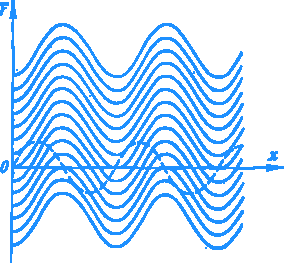
\includegraphics[width=0.6\textwidth]{figures/fig-44.pdf}
\caption{Graphs of the anti-derivatives of the function $f (x) = \sin x$.}
\label{fig-44}
\end{figure}

The figure clearly shows that all the antiderivatives belong to one family (in other words, correspond to the same initial function $f$). This may not always be as clear if the function is represented in an analytical form. Take, for
example, functions $F_{1} =-\cos x$ and $F_{2} =3- 2	\cos^{2} \dfrac{x}{2}$. It would be difficult to say at the first glance that these two
functions are the antiderivatives of \emph{one and the same function} (namely, $f = \sin x$). However, since $2 \cos^{2} \dfrac{x}{2} = 1 + cos x$, we find
\begin{equation*}%
F_{2}(x) = 3- 1 - \cos x =- \cos x + 2
\end{equation*}
\rdr I guess it would be possible to find directly that $F_{1}' (x) = F_{2}' (x)$, wouldn't it?

\athr Of course, it would:
\begin{align*}%
\ddx F_{2} (x) & = -2 \ddx \cos^{2} \dfrac{x}{2}  = 4 \cos \dfrac{x}{2} \sin \frac{x}{2} \cdot \frac{1}{2} = \sin x\\
& \\
\ddx F_{1} (x) & = \ddx (- \cos x) = \sin x
\end{align*}
But the easiest way is to notice that $F_{2} - F_{1} = C$. 

We could find numerous such examples. For instance, it is not difficult to check that the following pairs of functions belong to the same family of antiderivatives (each pair to its own family): 
\begin{enumerate}[label=(\alph*)]
\item $F_{1} = x^{2} - 2x + 3, \,\, F_{2} = (x- 1)^{2}$
\item $F_{1} = \arcsin x, \,\, F_{2} = 1 - \arccos x $
\item $F_{1} = \tan x \, \sin x + \cos x, \,\, F_{2} = (2 \cos x + 1) \dfrac{1}{ \cos x}$
\end{enumerate}
Thus, in case (a) we find $F_{2} -	F_{1} = -2$; both functions are the antiderivatives of the function $f = 2x - 2$.

Please, check cases (b) and (c) yourself. 

\rdr In case (b)  $F_{2} - F_{1} = (1 - \arccos x +
+ \arcsin x) = 1 - \dfrac{\pi}{2}$ both functions are the antiderivatives of the function $f = \dfrac{1}{1 - x^{2}}$

Case (c) is more intricate. Some preliminary manipulations are necessary:
\begin{align*}%
F_{1} (x) & = \tan x \sin x + \cos x = \dfrac{\sin^{2} x + \cos^{2} x}{\cos x} = \dfrac{1}{\cos x}\\
& \\
F_{2} (x) & = \frac{2 \cos x + 1 }{\cos x} = 2 + \dfrac{1}{\cos x}
\end{align*}
Therefore, $F_{2} - F_{1}=2$. Both functions ($F_{1}$ and $F_{2}$) are the antiderivatives of $f = \dfrac{\sin x}{\cos^{2} x}$

\athr Correct. Now, taking into account the results obtained in the previous dialogue, we can compile a table (see  \hyperref[deriv-list]{Table 2}) which gives various functions $f (x)$ in the first column the corresponding derivatives $f' (x)$ in the second column, and the antiderivatives $F (x) + C$, corresponding to the functions $f (x)$, in the third column. I want to stress once more: the transformation $f (x) \to f' (x)$ is the operation of differentiation of the function $f(x)$, and the transformation $f (x) \to [F (x) + C]$ is the operation of integration of the function $f (x)$.

\newpage 
%\vspace*{2cm}

\begin{center}
\textcolor{DodgerBlue}{\textbf{A List of Derivatives and Antiderivatives for Selected Functions}}\\[30pt]
%{\smaller
%\boxed{
\begin{tcolorbox}[colback=white,colframe=DodgerBlue]
\centering
\begin{tabular}{l>{\color{IndianRed}}r>{\color{IndianRed}}r>{\color{IndianRed}}r}
%\toprule
 & Function & Derivative & Antiderivative \\
  & $f(x)$ & $f'(x)$ &  F(x) \\
 \arrayrulecolor{DodgerBlue} \toprule
\circled{\rownumber} & $a$ & 0 & $ax + C$\\
    \arrayrulecolor{DodgerBlue}\midrule
\circled{\rownumber} & $x^{n}$ & $n x^{n-1}$ & $\dfrac{1}{n+1} x^{n+1} + C$\\
\midrule
\circled{\rownumber} & $e^{x}$ & $e^{x}$ & $e^{x} + C$\\
\midrule
\circled{\rownumber} & $\dfrac{1}{x}$ & $-\dfrac{1}{x^{2}}$ & $\ln x + C$\\
\midrule
\circled{\rownumber} & $\sqrt{x}$ &  $\dfrac{1}{2\sqrt{x}}$ & $\dfrac{2}{3} x  \sqrt{x} + C$\\
\midrule
\circled{\rownumber} & $\sin x$ & $\cos x$ & $- \cos x + C$\\
\midrule
\circled{\rownumber} & $\cos x$ & $-\sin x$ & $\sin x + C$\\
\midrule
\circled{\rownumber} & $\dfrac{1}{\cos^{2}} x$ & $2 \dfrac{\sin x}{\cos^{3} x}$ & $- \cot x + C$\\
\midrule
\circled{\rownumber} & $\dfrac{1}{\sin^{2} x}$ & $-2 \dfrac{\cos x}{\sin^{3} x}$ & $\tan x + C$\\
\midrule
\circled{\rownumber} & $\dfrac{1}{1 + x^{2}}$ & $-\dfrac{2 x}{ (1+x^{2})^{2}}$ & $\arctan x + C$\\
\label{deriv-list}
\end{tabular}
%}
\end{tcolorbox}
\end{center}

\newpage

\rdr Examples \circled{8}, \circled{9}, and \circled{10} in \hyperref[deriv-list]{Table 2} give an impression that the transformation $f (x) \to f' (x)$ is more complicated than the transformation $f (x) \to [F (x) + C]$.

\athr This impression stems from a special selection of the functions $f (x)$. Thus, it is easier to differentiate the function $\tan x$ than the function $\dfrac{1}{\cos^{2} x}$. Indeed, in the latter case we have to use the rules for differentiation of a ratio of two functions or of a composite function. 

In general, it should be noted that the operation of integration is substantially more complicated than that of differentiation. The differentiation of elementary functions invariably gives elementary functions. By employing the rules for differentiation discussed in the previous dialogue, you will be able (and with no difficulties, as a rule) to differentiate practically any elementary function. But integration is quite a different proposition. The rules for the integration of elementary functions comprise numerous techniques, and we would need several special dialogues to scan them. But the main point is that not every elementary function has an elementary function for its antiderivative. As one example, I shall mention the antiderivatives of such elementary
functions as $\dfrac{1}{\log x}$ or $\dfrac{1}{ \sqrt{1 + x^{2}}} $.
 As a rule, in such cases one is forced to resort to the methods of the so-called \emph{numerical integration}.

\rdr I was very attentive and want to pose two questions. First: What is meant by the term \emph{elementary function}?

\athr In \hyperref[derivative]{Dialogue Nine} I gave examples of the so-called \emph{fundamental elementary functions} ($x^{n}, \, x^{-n}, \, x^{1/n}, \, \sin x, \, \cos x,$ $\,	\tan x, \,	\cot x,	\, \arcsin x,$ $\,	\arccos x,	\, \arctan x, \,	\arccot x, \, a^{x}, \, \log_{a} x$]. An \emph{elementary function} is any function which can be formed of \emph{fundamental elementary functions} by a \emph{finite} number of the operations of addition, subtraction, multiplication, division, involution, evolution, and taking a modulus, as well as by using the rules for obtaining inverse and composite functions. All the functions used in the previous dialogues are elementary (with an exception of the Dirichlet function mentioned in \hyperref[{more-on-function}]{Dialogue Five}), and many of them are fundamental elementary functions.

\rdr My second question concerns the \emph{rules for integration} you refer to. Could you give at least some examples?

\athr I shall quote three simplest rules.
\begin{mytheo}{Three Simple Rules for Integration}
\begin{enumerate}[label=\protect\circled{\arabic*}]
\item If $F$ is an antiderivative for $f$. and $G$ is an anti-derivative for $g$, an antiderivative for the sum of the functions $f + g$ is a function $F + G$.
\item If $F$ is an antiderivative for $f$ an antiderivative for a function $af$, where $a$ is a constant, is a function $aF$.
\item If $F (x)$ is an antiderivative for $f (x)$, and $a$ and $b$ are constants, an antiderivative for a function $f (ax + b)$ is a function $\dfrac{1}{a} F (ax + b)$.
\end{enumerate}
\end{mytheo}
All the three rules are proved readily by using the rules for differentiation (in the third rule one has to apply the rule for the differentiation of composite functions). Indeed,
\begin{enumerate}[label=\protect\circled{\arabic*}]
\item $\ddx (F+G) = \ddx F + \ddx G= f + g$ 
\item $\ddx (aF)= a \ddx F= af$
\item $\begin{aligned}[t]%
\ddx \left( \frac{1}{a} F (ax + b)  \right)  & = \frac{1}{a} \ddx F(ax +b) =  \frac{1}{a} \dfrac{d}{dy} F(y) \ddx (ax +b) \\
& =  \frac{1}{a} f(y)\, a = f(y) = f(ax +b) 
\\ & \text{here:} \,\, y = ax +b
\end{aligned}$
\end{enumerate}
Of course, the three rules cited above do not exhaust a rich collection of integration rules available in calculus. 

But here these three rules will be sufficient since our goal is quite modest: to give the fundamental idea of an anti-derivative.

\rdr Our discussion of a derivative covered its geometrical interpretation as well. Is there a geometrical  interpretation of an antiderivative?

\athr Yes, there is. Let us find it (besides, we shall need it later).

Consider a function $f (x)$. For the sake of simplicity, assume that this function is \emph{monotonic} (and even \emph{increasing}). Later we shall drop the monotonicity of a function. The most important is that the function be \emph{continuous} over the chosen interval (i.e. over the interval on which it is defined). \fig{fig-45} shows a shaded area (the so-called \emph{curvilinear trapezoid}) bounded by the graph of the function $f (x)$, the interval $[a, x]$ of the $x$-axis, and two perpendiculars	erected from points $a$ and $x$ on the $x$-axis. Let point $a$ be fixed; as for point $x$ (the right-hand end of the interval $[a, \, x]$), it is not fixed and can assume values from a upward (within the domain of definition of the function). Obviously, the \emph{area} of the curvilinear trapezoid shaded in the figure is a \emph{function} of $x$. We shall denote it by $S (x)$,

\begin{figure}[!ht]%[13]{r}{0.5\textwidth}
\centering
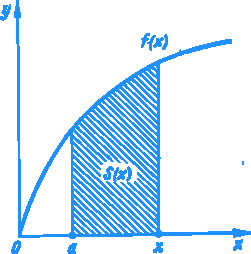
\includegraphics[width=0.5\textwidth]{figures/fig-45.pdf}
\caption{Examining the geometrical interpretation of the antiderivative.}
\label{fig-45}
\end{figure}

Now turn to \fig{fig-46}. Let us give an increment $\Delta x$ to the independent variable $x$. The interval $[a, \, x + \Delta x]$ corresponds to the area $S (x + \Delta x)$. Denote $\Delta S(x) = S (x + \Delta x)- S (x)$. The increment $\Delta S(x)$ is, obviously, the area of the shaded curvilinear trapezoid. The figure shows that
\begin{equation*}%
\text{area} \,\, ADEF < \Delta S (x) < \text{area} \,\, ABCF 
\end{equation*}

\begin{figure}[!ht]%[13]{r}{0.5\textwidth}
\centering
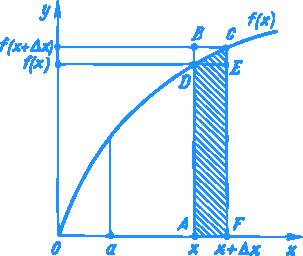
\includegraphics[width=0.6\textwidth]{figures/fig-46.pdf}
\caption{Examining the geometrical interpretation of the antiderivative.}
\label{fig-46}
\end{figure}

But the area $ADEF$ is equal to $f (x) \Delta x$, and the area $ABCF$
is equal to $f (x +  \Delta x) \Delta x$. Therefore,
\begin{equation*}%
\text{area} \,\, ADEF < \Delta S (x) < \text{area} \,\, ABCF 
\end{equation*}
or
\begin{equation*}%
f (x) \Delta x < \dfrac{\Delta S (x)}{ \Delta x}  < f (x + \Delta x)
\end{equation*}
or
\begin{equation*}%
0 < \left(  \dfrac{\Delta S (x)}{ \Delta x}  - f (x) \right) < [f (x) + \Delta x)-	f (x)] = \Delta f(x) 
\end{equation*}

Now we find the limiting values of these inequalities for $\Delta x$ tending to zero. By virtue of the continuity of the function $f (x)$ we conclude that $\lmts{\Delta x}{0} \Delta f (x) = 0$. Consequently,
\begin{equation*}%
\lmts{\Delta x}{0} \left(  \dfrac{\Delta S (x)}{ \Delta x}  - f (x) \right) = 0
\end{equation*}
As the function $f (x)$ is independent of $\Delta x$, the last relation yields
\begin{equation}%
\lmts{\Delta x}{0}  \dfrac{\Delta S (x)}{ \Delta x}  = f (x)
\label{antideriv-geom1}
%eq 2 of 11
\end{equation}
By the definition of derivative,
\begin{equation*}%
\lmts{\Delta x}{0}  \dfrac{\Delta S (x)}{ \Delta x}  = S' (x)
\end{equation*}
Consequently, relation \eqref{antideriv-geom1} signifies that
\begin{equation}%
 f (x)  = S' (x)
\label{antideriv-geom2}
%eq 3 of 11
\end{equation}

Thus, in terms of geometry, \emph{the antiderivative of the function $f$, taken at point $x$, is the area of curvilinear trapezoid bounded by the graph of the function $f (x)$ over the interval $[a, x]$ of the $x$-axis}.

\rdr Presumably, it is one of the possible anti-derivatives, isn't it?

\athr Definitely.

\rdr But it is evident that the area $S (x)$ also depends on the choice of point $a$.

\athr Absolutely correct. By choosing different points $a$, we shall have different areas of curvilinear trapezoids and, correspondingly, different antiderivatives. But all of them will be the antiderivatives of the function $f$ taken at point $x$. It is only important that in all cases $a < x$.

\rdr Then why is it that point $a$ vanishes from the final results?

\athr Your bewilderment is understandable. Let us reformulate the results obtained above. Let $F (x)$ be an antiderivative of a function $f (x)$ taken at point $x$. According to \eqref{antideriv-geom2}, we can write
\begin{equation*}%
S(x) = F(x) + C
\end{equation*}
(here we have used the following theorem: if two functions have equal derivatives, the functions will differ by a constant term). The constant $C$ is found readily since $S (a) = 0$. Therefore,
\begin{equation*}%
S (a) = F (a) + C = 0
\end{equation*}
Hence, $C = -F (a)$. This gives
\begin{equation}%
S(x)=F(x)- F(a)
\label{antideriv-geom3}
%eq 4 of 11
\end{equation}

\begin{mytheo}{Conclusion}
If $F (x)$ is an antiderivative of a function $f (x)$, then the area $S (x)$ of a curvilinear trapezoid bounded by the graph of the junction $f (x)$ over the interval $[a, x]$ is given by the difference $F (x)- F (a)$.
\end{mytheo}
You see now that point $a$ is introduced explicitly. 

\rdr Now everything is clear, 

\athr Relation \eqref{antideriv-geom2} (and from it, \eqref{antideriv-geom3}) can be obtained for every continuous function; the \emph{monotonicity} of a function is \emph{not} a necessary condition. Consider a function $f (x)$ whose graph is plotted in \fig{fig-47}. We choose a point $x$ and wish to prove that for any $\varepsilon > 0$ there is $\delta > 0 $ such that
\begin{equation}%
\left|  \dfrac{\Delta S (x)}{ \Delta x}   - f(x) \right| < \varepsilon
\label{antideriv-geom4}
%eq 5 of 11
\end{equation}

for all $\Delta x$ satisfying the condition $| \Delta x |<  \delta$. 

\begin{figure}[!ht]%[13]{r}{0.5\textwidth}
\centering
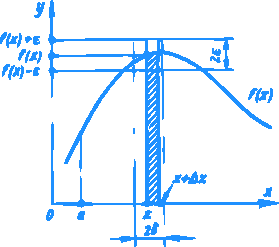
\includegraphics[width=0.6\textwidth]{figures/fig-47.pdf}
\caption{Examining the geometrical interpretation of the antiderivative.}
\label{fig-47}
\end{figure}

\rdr Shall we consider point $x$ as fixed? 

\athr Yes. Increments $\Delta x$ and, correspondingly,
$\Delta S (x)$, are always considered for a definite point $x$.
So we take an arbitrary number $\varepsilon > 0$ (shown in the figure).  As f (x) is a continuous function, there is a number $\delta > 0$ such that 
\begin{equation}%
|f(x) + \Delta x - f(x)| < \varepsilon
\label{antideriv-geom5}
%eq 6 of 11
\end{equation}
for all $\Delta x$ satisfying the condition $| \Delta x | < 0$. This number $\delta$ is the one we were to find.

Indeed, let us choose, for definiteness, that $\Delta x > 0$ but specify that $\Delta x < \delta$. The area of the curvilinear trapezoid shaded in \fig{fig-47} will be denoted by $\Delta S (x)$ (this trapezoid is bounded by the graph of the function $f (x)$ over the interval $[x, \, x + \Delta x]$. Inequality \eqref{antideriv-geom5} yields (see the figure):
\begin{equation*}%
[f(x)  -   \varepsilon] \Delta x < \Delta S (x) < [f(x) - \varepsilon] \Delta x
\end{equation*}
or
\begin{equation*}%
[f(x)  -   \varepsilon]  < \dfrac{\Delta S (x)}{\Delta x} < [f(x) - \varepsilon]
\end{equation*}
or, 
\begin{equation*}%
 -  \varepsilon < \left( \dfrac{\Delta S (x)}{\Delta x} - f(x) \right)  < \varepsilon 
\end{equation*}
or, finally.
\begin{equation*}%
\left| \dfrac{\Delta S (x)}{\Delta x} - f(x) \right|  < \varepsilon
\end{equation*}
which is what we wanted to prove.

You see that a function $f$ needn't be monotonic: relation \eqref{antideriv-geom2} (and with it, \eqref{antideriv-geom3} is easily generalized to the case of an arbitrary continuous function $f$.

Now let us turn again to \fig{fig-44} that gives a family of graphs of the antiderivative $F (x) = - \cos x + C$ for the function $f (x) = \sin x$. Indicate which of these graphs (which antiderivative) stands for $S (x)$ in each of the following three cases: 
\begin{enumerate*}[label=(\alph*)]
\item $a = 0$, 
\item $a = \dfrac{\pi}{2}$, and 
\item $a = \pi$. 
\end{enumerate*}

\rdr The question is clear. I denote the sought functions	by	$S_{1} (x), \, S_{2}	(x)$, and $ S_{3} (x)$, respectively.	These functions are plotted in \fig{fig-48}.

Obviously, we can write
\begin{align*}%
S_{1}(x) & = F(x) - F(0) \\
S_{2}(x) & = F(x) - F(\dfrac{\pi}{2})\\
S_{3}(x) &= F(x) - F(\pi)
\end{align*}

\athr  Correct. It is important to underline that in each of the above three equalities the function $F (x)$ is a function chosen arbitrarily from the family of antiderivatives of $f$, shown in \fig{fig-44}.

\begin{figure}[!ht]%[13]{r}{0.5\textwidth}
\centering
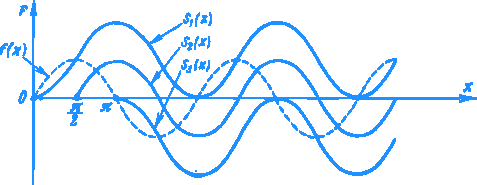
\includegraphics[width=\textwidth]{figures/fig-48.pdf}
\caption{Particular graphs of the antiderivative for specific value of $a$.}
\label{fig-48}
\end{figure}

\rdr It looks as if whatever the selected antiderivative of the function $f$ is, the difference between its values at two points depends only on the choice of these points but not on the choice of a specific antiderivative.

\athr You have pointed out a property of principal significance. It is so important that deserves a special dialogue.